% !TEX root = /home/computer/ucsc/master-2/quarter-1/computational-fluids/master.tex
\assignment{4}{Fri 19 Nov 2021 12:48}{Project}

\subsectionfont{\fontsize{10}{10}\selectfont}

\graphicspath{{./assignment_04/figures/}}

\section{Sod's Shock Tube $\gamma = 1.4$, $t = 0.2$}%
Using various limiters for HLL

\[
V(x,0) =
\begin{cases}
 \begin{pmatrix}
   1.0 \\ -2.0 \\ 0.4
 \end{pmatrix}_L & x \leq 0.5, \\\\
 \begin{pmatrix}
   1.0 \\ 2.0 \\ 1.0 
 \end{pmatrix}_R & x > 0.5, \\
\end{cases}
.\] 

\subsection{Non-conservative limiters}%


\begin{figure}[H]
  \centering
  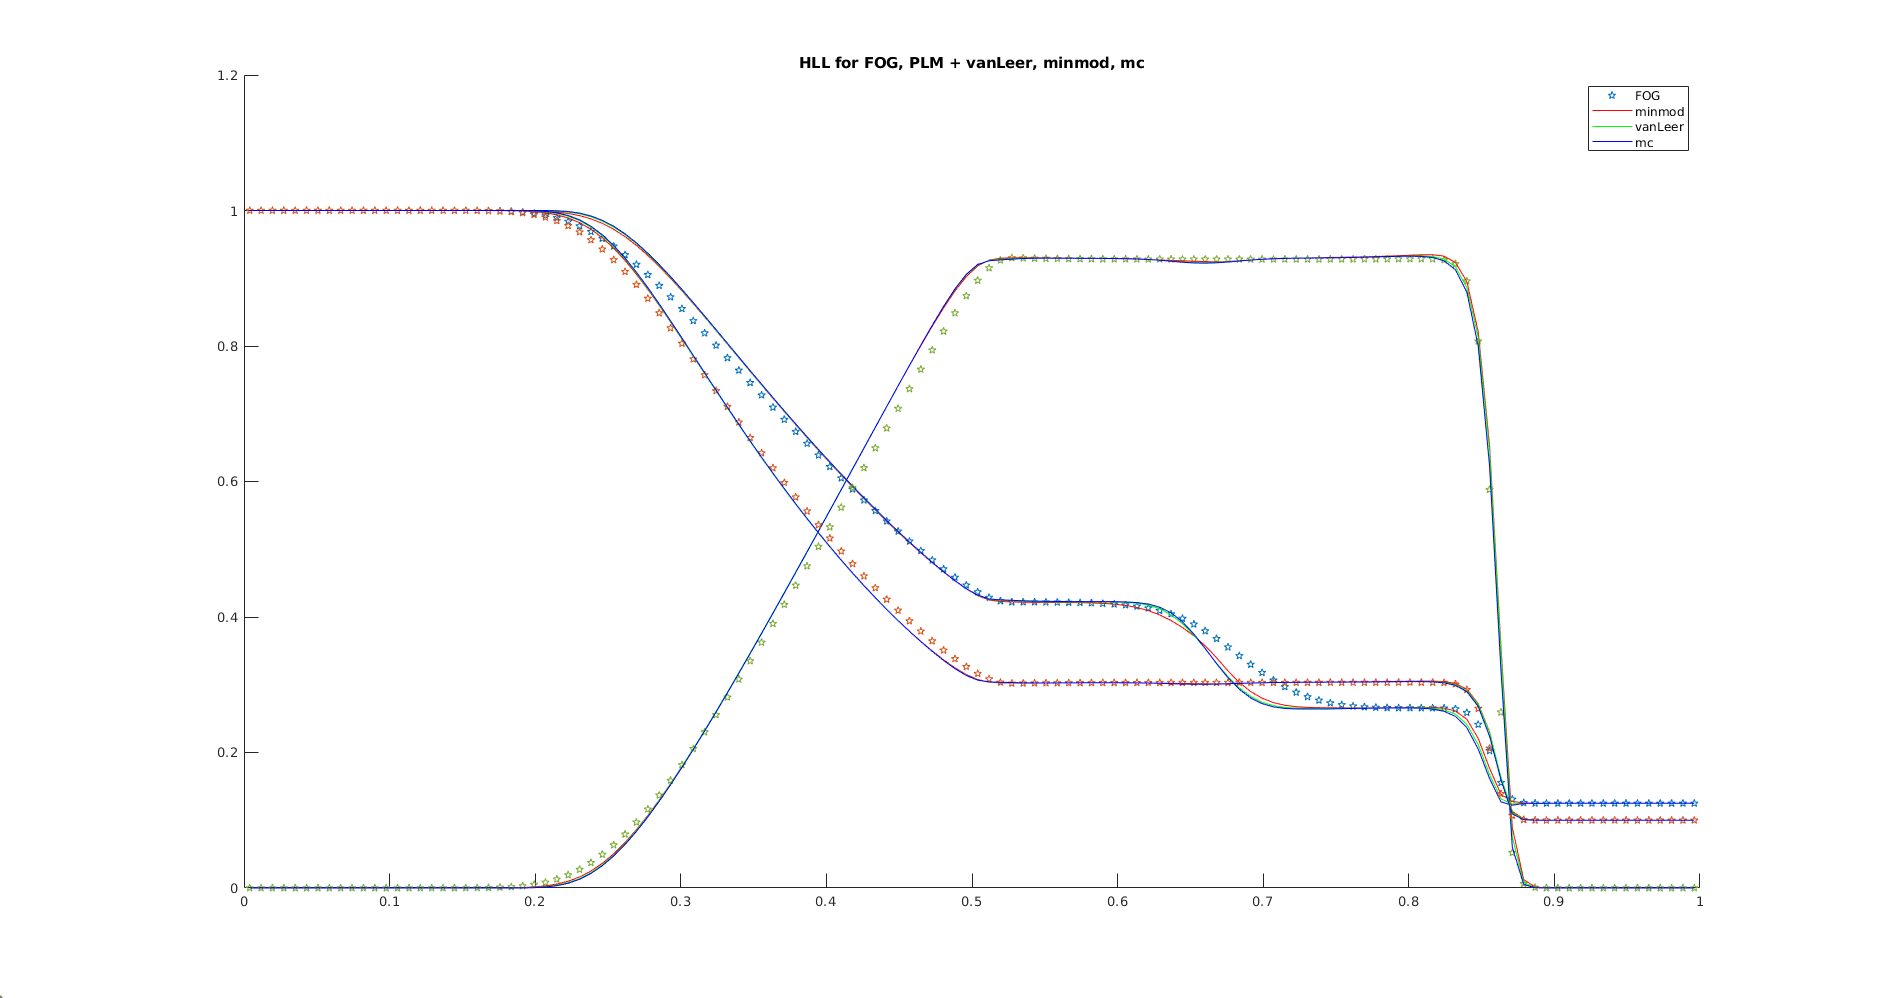
\includegraphics[width=0.8\linewidth]{HLL1false.png}
  \caption{L1false}%
  \label{fig:L1false}
\end{figure}

\subsection{Conservative limiters}%

\begin{figure}[H]
  \centering
  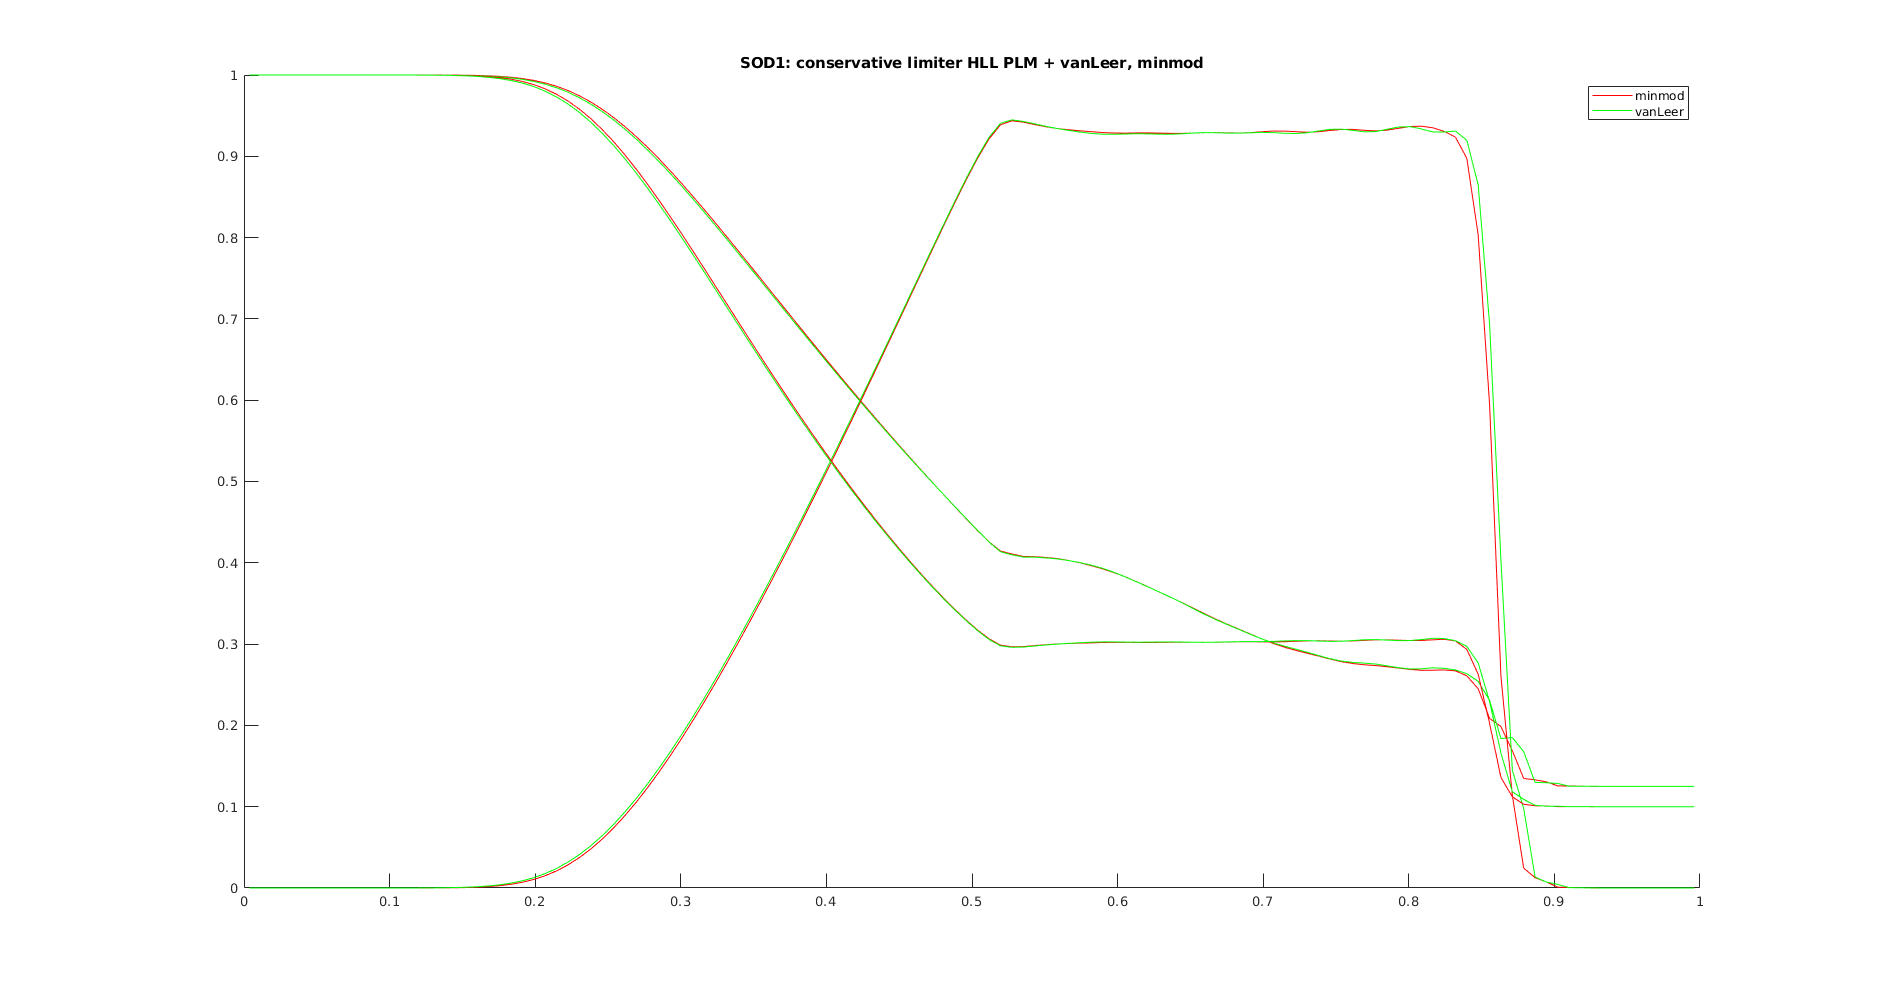
\includegraphics[width=0.8\linewidth]{consLimHLL.png}
  \caption{ConsLimHLL}%
  \label{fig:consLimHLL}
\end{figure}

\section{Rarefaction $\gamma = 1.4$, $t = 0.15$}%

Using various limiters for HLL
\[
V(x,0) =
\begin{cases}
 \begin{pmatrix}
   1.0 \\ -2.0 \\ 0.4
 \end{pmatrix}_L & x \leq 0.5, \\\\
 \begin{pmatrix}
   1.0 \\ 2.0 \\ 1.0 
 \end{pmatrix}_R & x > 0.5, \\
\end{cases}
.\] 

\begin{figure}[H]
  \centering
  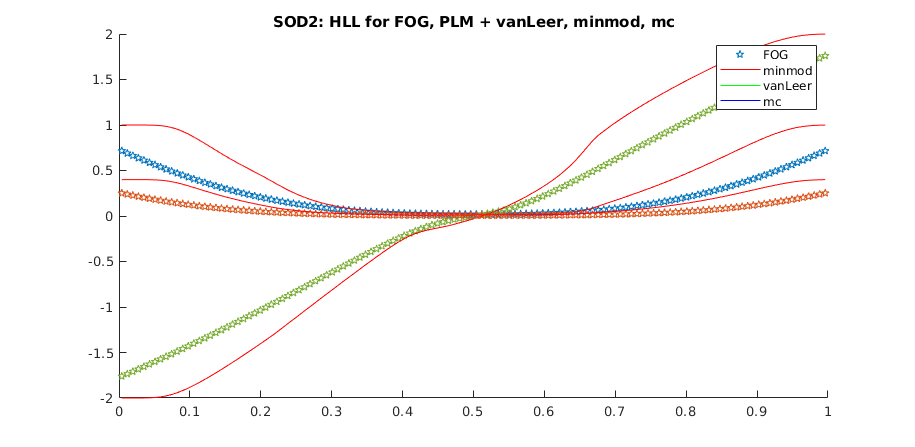
\includegraphics[width=0.8\linewidth]{HLL2false.png}
  \caption{L2false}%
  \label{fig:L2false}
\end{figure}
